\documentclass[twoside]{book}

% Packages required by doxygen
\usepackage{calc}
\usepackage{doxygen}
\usepackage{graphicx}
\usepackage[utf8]{inputenc}
\usepackage{makeidx}
\usepackage{multicol}
\usepackage{multirow}
\usepackage{textcomp}
\usepackage[table]{xcolor}

% Font selection
\usepackage[T1]{fontenc}
\usepackage{mathptmx}
\usepackage[scaled=.90]{helvet}
\usepackage{courier}
\usepackage{amssymb}
\usepackage{sectsty}
\renewcommand{\familydefault}{\sfdefault}
\allsectionsfont{%
  \fontseries{bc}\selectfont%
  \color{darkgray}%
}
\renewcommand{\DoxyLabelFont}{%
  \fontseries{bc}\selectfont%
  \color{darkgray}%
}

% Page & text layout
\usepackage{geometry}
\geometry{%
  a4paper,%
  top=2.5cm,%
  bottom=2.5cm,%
  left=2.5cm,%
  right=2.5cm%
}
\tolerance=750
\hfuzz=15pt
\hbadness=750
\setlength{\emergencystretch}{15pt}
\setlength{\parindent}{0cm}
\setlength{\parskip}{0.2cm}
\makeatletter
\renewcommand{\paragraph}{%
  \@startsection{paragraph}{4}{0ex}{-1.0ex}{1.0ex}{%
    \normalfont\normalsize\bfseries\SS@parafont%
  }%
}
\renewcommand{\subparagraph}{%
  \@startsection{subparagraph}{5}{0ex}{-1.0ex}{1.0ex}{%
    \normalfont\normalsize\bfseries\SS@subparafont%
  }%
}
\makeatother

% Headers & footers
\usepackage{fancyhdr}
\pagestyle{fancyplain}
\fancyhead[LE]{\fancyplain{}{\bfseries\thepage}}
\fancyhead[CE]{\fancyplain{}{}}
\fancyhead[RE]{\fancyplain{}{\bfseries\leftmark}}
\fancyhead[LO]{\fancyplain{}{\bfseries\rightmark}}
\fancyhead[CO]{\fancyplain{}{}}
\fancyhead[RO]{\fancyplain{}{\bfseries\thepage}}
\fancyfoot[LE]{\fancyplain{}{}}
\fancyfoot[CE]{\fancyplain{}{}}
\fancyfoot[RE]{\fancyplain{}{\bfseries\scriptsize Generated on Mon Mar 16 2015 16\-:31\-:26 for Bixel by Doxygen }}
\fancyfoot[LO]{\fancyplain{}{\bfseries\scriptsize Generated on Mon Mar 16 2015 16\-:31\-:26 for Bixel by Doxygen }}
\fancyfoot[CO]{\fancyplain{}{}}
\fancyfoot[RO]{\fancyplain{}{}}
\renewcommand{\footrulewidth}{0.4pt}
\renewcommand{\chaptermark}[1]{%
  \markboth{#1}{}%
}
\renewcommand{\sectionmark}[1]{%
  \markright{\thesection\ #1}%
}

% Indices & bibliography
\usepackage{natbib}
\usepackage[titles]{tocloft}
\setcounter{tocdepth}{3}
\setcounter{secnumdepth}{5}
\makeindex

% Hyperlinks (required, but should be loaded last)
\usepackage{ifpdf}
\ifpdf
  \usepackage[pdftex,pagebackref=true]{hyperref}
\else
  \usepackage[ps2pdf,pagebackref=true]{hyperref}
\fi
\hypersetup{%
  colorlinks=true,%
  linkcolor=blue,%
  citecolor=blue,%
  unicode%
}

% Custom commands
\newcommand{\clearemptydoublepage}{%
  \newpage{\pagestyle{empty}\cleardoublepage}%
}


%===== C O N T E N T S =====

\begin{document}

% Titlepage & ToC
\hypersetup{pageanchor=false}
\pagenumbering{roman}
\begin{titlepage}
\vspace*{7cm}
\begin{center}%
{\Large Bixel }\\
\vspace*{1cm}
{\large Generated by Doxygen 1.8.6}\\
\vspace*{0.5cm}
{\small Mon Mar 16 2015 16:31:26}\\
\end{center}
\end{titlepage}
\clearemptydoublepage
\tableofcontents
\clearemptydoublepage
\pagenumbering{arabic}
\hypersetup{pageanchor=true}

%--- Begin generated contents ---
\chapter{Todo List}
\label{todo}
\hypertarget{todo}{}

\begin{DoxyRefList}
\item[\label{todo__todo000003}%
\hypertarget{todo__todo000003}{}%
Member \hyperlink{classBixelGrid_a3980df6f8699db73452b0893190877ce}{Bixel\-Grid\-:\-:decrease\-Dimension} ()]Get rid of this. See the todos in \#increase\-Dimension.  
\item[\label{todo__todo000001}%
\hypertarget{todo__todo000001}{}%
Member \hyperlink{classBixelGrid_aac761dbec07e93c105dd7332e982698c}{Bixel\-Grid\-:\-:dimension} ()]Get rid of this. See \#increase\-Dimension todos.  
\item[\label{todo__todo000005}%
\hypertarget{todo__todo000005}{}%
Member \hyperlink{classBixelGrid_a2f45709d9159599eb3af5ceed54fc550}{Bixel\-Grid\-:\-:Draw\-Tool} ]Move H\-A\-N\-D and Z\-O\-O\-M to an enum in \hyperlink{classCanvasWidget}{Canvas\-Widget}. 

Implement E\-Y\-E\-D\-R\-O\-P 

Add a Paint\-Bucket tool. 

Add a Magic wand tool. 

Flesh out tools enum documentation  
\item[\label{todo__todo000002}%
\hypertarget{todo__todo000002}{}%
Member \hyperlink{classBixelGrid_a589e8542077e6afea967a85e8d040298}{Bixel\-Grid\-:\-:increase\-Dimension} ()]The way I have been dealing with \#dimension is ridiculous. Get rid of m\-\_\-dimension altogether and use only \#grid\-Width and \#grid\-Height. Create an increase\-Width() and an increase\-Height() as well as a decrease\-Width/\-Height.  
\item[\label{todo__todo000006}%
\hypertarget{todo__todo000006}{}%
Member \hyperlink{classBixelGrid_a2f45709d9159599eb3af5ceed54fc550aa9b97045f133062453e585409323d940}{Bixel\-Grid\-:\-:P\-A\-I\-N\-T\-B\-U\-C\-K\-E\-T} ]implement this  
\item[\label{todo__todo000004}%
\hypertarget{todo__todo000004}{}%
Member \hyperlink{classBixelGrid_a5ddc685a7df1db41dd1716e03342d619}{Bixel\-Grid\-:\-:paint\-G\-L} ()]Give Bixel drawing work to Open\-G\-L. Use one Mesh instead of many calls to G\-L\-\_\-\-D\-R\-A\-W\-\_\-\-A\-R\-R\-A\-Y\-S  
\item[\label{todo__todo000007}%
\hypertarget{todo__todo000007}{}%
Class \hyperlink{classBixelWindow}{Bixel\-Window} ]Figure out how to keep focus on gl\-Widget. Maybe make al gl\-Widget keyboard actions Q\-Actions in the menu? 
\end{DoxyRefList}
\chapter{Hierarchical Index}
\section{Class Hierarchy}
This inheritance list is sorted roughly, but not completely, alphabetically\-:\begin{DoxyCompactList}
\item \contentsline{section}{Bixel\-Grid\-:\-:History\-State}{\pageref{structBixelGrid_1_1HistoryState}}{}
\item Q\-G\-L\-Widget\begin{DoxyCompactList}
\item \contentsline{section}{Bixel\-Grid}{\pageref{classBixelGrid}}{}
\end{DoxyCompactList}
\item Q\-Main\-Window\begin{DoxyCompactList}
\item \contentsline{section}{Bixel\-Window}{\pageref{classBixelWindow}}{}
\end{DoxyCompactList}
\item Q\-Tool\-Button\begin{DoxyCompactList}
\item \contentsline{section}{Swatch}{\pageref{classSwatch}}{}
\end{DoxyCompactList}
\item Q\-Widget\begin{DoxyCompactList}
\item \contentsline{section}{Canvas\-Widget}{\pageref{classCanvasWidget}}{}
\end{DoxyCompactList}
\item \contentsline{section}{vec2}{\pageref{classvec2}}{}
\end{DoxyCompactList}

\chapter{Class Index}
\section{Class List}
Here are the classes, structs, unions and interfaces with brief descriptions\-:\begin{DoxyCompactList}
\item\contentsline{section}{\hyperlink{classBixelWindow}{Bixel\-Window} }{\pageref{classBixelWindow}}{}
\item\contentsline{section}{\hyperlink{classCanvasWidget}{Canvas\-Widget} }{\pageref{classCanvasWidget}}{}
\item\contentsline{section}{\hyperlink{classGLWidget}{G\-L\-Widget} \\*A Widget for rendering and drawing Bixels }{\pageref{classGLWidget}}{}
\item\contentsline{section}{\hyperlink{structGLWidget_1_1HistoryState}{G\-L\-Widget\-::\-History\-State} \\*This struct stores the current state of a \hyperlink{classGLWidget}{G\-L\-Widget} }{\pageref{structGLWidget_1_1HistoryState}}{}
\item\contentsline{section}{\hyperlink{classSwatch}{Swatch} }{\pageref{classSwatch}}{}
\item\contentsline{section}{\hyperlink{classvec2}{vec2} }{\pageref{classvec2}}{}
\end{DoxyCompactList}

\chapter{Class Documentation}
\input{classBixelGrid}
\hypertarget{classBixelWindow}{\section{Bixel\-Window Class Reference}
\label{classBixelWindow}\index{Bixel\-Window@{Bixel\-Window}}
}


{\ttfamily \#include $<$bixelwindow.\-hpp$>$}



Inheritance diagram for Bixel\-Window\-:\nopagebreak
\begin{figure}[H]
\begin{center}
\leavevmode
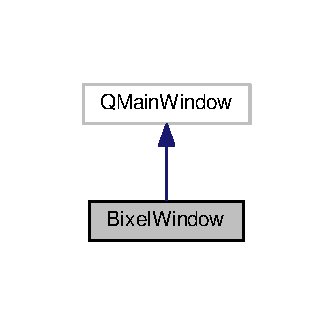
\includegraphics[width=160pt]{classBixelWindow__inherit__graph}
\end{center}
\end{figure}


Collaboration diagram for Bixel\-Window\-:\nopagebreak
\begin{figure}[H]
\begin{center}
\leavevmode
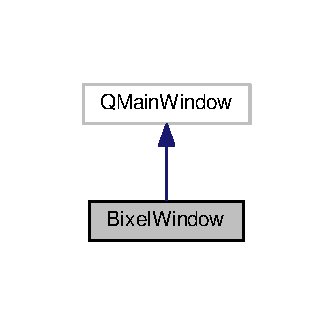
\includegraphics[width=160pt]{classBixelWindow__coll__graph}
\end{center}
\end{figure}
\subsection*{Public Slots}
\begin{DoxyCompactItemize}
\item 
\hypertarget{classBixelWindow_a4cb74f4db84d75a09598acba37f97268}{void {\bfseries open\-\_\-slot} (std\-::string file\-Name)}\label{classBixelWindow_a4cb74f4db84d75a09598acba37f97268}

\end{DoxyCompactItemize}
\subsection*{Signals}
\begin{DoxyCompactItemize}
\item 
\hypertarget{classBixelWindow_a0ca7305900c3368348c36dbd73a51af9}{void {\bfseries new\-\_\-file\-\_\-signal} ()}\label{classBixelWindow_a0ca7305900c3368348c36dbd73a51af9}

\item 
\hypertarget{classBixelWindow_ac3542a30d554c494749f81c4928e4691}{void {\bfseries save\-\_\-signal} ()}\label{classBixelWindow_ac3542a30d554c494749f81c4928e4691}

\item 
\hypertarget{classBixelWindow_a184916c5970b4189571c61a40bcddb81}{void {\bfseries save\-\_\-as\-\_\-signal} (const std\-::string \&file\-Name)}\label{classBixelWindow_a184916c5970b4189571c61a40bcddb81}

\item 
\hypertarget{classBixelWindow_a1f5cdec267152e7c84fa3430c4cea442}{void {\bfseries open\-\_\-signal} (const std\-::string \&file\-Name)}\label{classBixelWindow_a1f5cdec267152e7c84fa3430c4cea442}

\item 
\hypertarget{classBixelWindow_a64703a78a6b4e436248dbed135fe5420}{void {\bfseries export\-\_\-image\-\_\-signal} (const std\-::string \&file\-Name)}\label{classBixelWindow_a64703a78a6b4e436248dbed135fe5420}

\item 
\hypertarget{classBixelWindow_af52996e623d4b53b5dc905c931960dc1}{void {\bfseries preferences\-\_\-signal} ()}\label{classBixelWindow_af52996e623d4b53b5dc905c931960dc1}

\item 
\hypertarget{classBixelWindow_a94c52d6d03787661d8cb142657cfebbd}{void {\bfseries undo\-\_\-signal} ()}\label{classBixelWindow_a94c52d6d03787661d8cb142657cfebbd}

\item 
\hypertarget{classBixelWindow_aaec5ff0c79673adf41f9d11acf8d696d}{void {\bfseries redo\-\_\-signal} ()}\label{classBixelWindow_aaec5ff0c79673adf41f9d11acf8d696d}

\item 
\hypertarget{classBixelWindow_a752d221cb9e200ee23a3ad0cf20fd8b8}{void {\bfseries copy\-\_\-signal} ()}\label{classBixelWindow_a752d221cb9e200ee23a3ad0cf20fd8b8}

\item 
\hypertarget{classBixelWindow_a1fe8ae25f04273997c5b23bbb161af4e}{void {\bfseries cut\-\_\-signal} ()}\label{classBixelWindow_a1fe8ae25f04273997c5b23bbb161af4e}

\item 
\hypertarget{classBixelWindow_a587d0745d036eabace33de931104d4c7}{void {\bfseries paste\-\_\-signal} ()}\label{classBixelWindow_a587d0745d036eabace33de931104d4c7}

\item 
\hypertarget{classBixelWindow_a42b6e8b3cc3f837a6233c616ea26a9c4}{void {\bfseries select\-\_\-all\-\_\-signal} ()}\label{classBixelWindow_a42b6e8b3cc3f837a6233c616ea26a9c4}

\item 
\hypertarget{classBixelWindow_a5e64c14663eadc91c7c6015d4981fb70}{void {\bfseries deselect\-\_\-all\-\_\-signal} ()}\label{classBixelWindow_a5e64c14663eadc91c7c6015d4981fb70}

\item 
\hypertarget{classBixelWindow_a119d72d0e838a8d3689a3adecd4525e4}{void {\bfseries reset\-\_\-view\-\_\-signal} ()}\label{classBixelWindow_a119d72d0e838a8d3689a3adecd4525e4}

\item 
\hypertarget{classBixelWindow_a3905766a93b07f84fb2a42bf06d83f06}{void {\bfseries zoom\-\_\-in\-\_\-signal} ()}\label{classBixelWindow_a3905766a93b07f84fb2a42bf06d83f06}

\item 
\hypertarget{classBixelWindow_afe6f72f82acd783d9a558b7c0e320dd3}{void {\bfseries zoom\-\_\-out\-\_\-signal} ()}\label{classBixelWindow_afe6f72f82acd783d9a558b7c0e320dd3}

\item 
\hypertarget{classBixelWindow_a8b65e3840cb126f9d38d4edf7df0eba9}{void {\bfseries custom\-\_\-zoom\-\_\-signal} ()}\label{classBixelWindow_a8b65e3840cb126f9d38d4edf7df0eba9}

\end{DoxyCompactItemize}
\subsection*{Public Member Functions}
\begin{DoxyCompactItemize}
\item 
\hypertarget{classBixelWindow_ae334b79d3ae7e7dbd9a967c5a4281fdc}{{\bfseries Bixel\-Window} (Q\-Widget $\ast$parent=0, Qt\-::\-Window\-Flags flags=0)}\label{classBixelWindow_ae334b79d3ae7e7dbd9a967c5a4281fdc}

\end{DoxyCompactItemize}
\subsection*{Public Attributes}
\begin{DoxyCompactItemize}
\item 
\hypertarget{classBixelWindow_a244d329ec6f85ab43a997063be46dea2}{Q\-Action $\ast$ {\bfseries new\-\_\-file}}\label{classBixelWindow_a244d329ec6f85ab43a997063be46dea2}

\item 
\hypertarget{classBixelWindow_a0a042b7df3f5c5f894129d389c9954ec}{Q\-Action $\ast$ {\bfseries save}}\label{classBixelWindow_a0a042b7df3f5c5f894129d389c9954ec}

\item 
\hypertarget{classBixelWindow_ac9e04ce9181d3f46d36079aace0df10f}{Q\-Action $\ast$ {\bfseries save\-\_\-as}}\label{classBixelWindow_ac9e04ce9181d3f46d36079aace0df10f}

\item 
\hypertarget{classBixelWindow_ac354692478ee5930348b3671d8637ed0}{Q\-Action $\ast$ {\bfseries open}}\label{classBixelWindow_ac354692478ee5930348b3671d8637ed0}

\item 
\hypertarget{classBixelWindow_af2c2cd235d976dc607a49bac00722a0f}{Q\-Action $\ast$ {\bfseries export\-\_\-image}}\label{classBixelWindow_af2c2cd235d976dc607a49bac00722a0f}

\item 
\hypertarget{classBixelWindow_aa49b259412ee513d078340ddd767196b}{Q\-Action $\ast$ {\bfseries preferences}}\label{classBixelWindow_aa49b259412ee513d078340ddd767196b}

\item 
\hypertarget{classBixelWindow_a1989fb441499dab98383bc8eece8cb57}{Q\-Action $\ast$ {\bfseries undo}}\label{classBixelWindow_a1989fb441499dab98383bc8eece8cb57}

\item 
\hypertarget{classBixelWindow_af0af99759611ce859f7656ae6a8dd344}{Q\-Action $\ast$ {\bfseries redo}}\label{classBixelWindow_af0af99759611ce859f7656ae6a8dd344}

\item 
\hypertarget{classBixelWindow_aaa17e3ee8a780e8dc872a05f4a417bbf}{Q\-Action $\ast$ {\bfseries copy}}\label{classBixelWindow_aaa17e3ee8a780e8dc872a05f4a417bbf}

\item 
\hypertarget{classBixelWindow_af629761b1bf39d792ae05ed7f8752627}{Q\-Action $\ast$ {\bfseries cut}}\label{classBixelWindow_af629761b1bf39d792ae05ed7f8752627}

\item 
\hypertarget{classBixelWindow_af9f9f91f2811d896822857a55a7ec172}{Q\-Action $\ast$ {\bfseries paste}}\label{classBixelWindow_af9f9f91f2811d896822857a55a7ec172}

\item 
\hypertarget{classBixelWindow_a279e6e5b9f5c435dad5049260bf12a13}{Q\-Action $\ast$ {\bfseries select\-\_\-all}}\label{classBixelWindow_a279e6e5b9f5c435dad5049260bf12a13}

\item 
\hypertarget{classBixelWindow_ac86dc4f1dd11518d9ecb31d65a5a74f5}{Q\-Action $\ast$ {\bfseries deselect\-\_\-all}}\label{classBixelWindow_ac86dc4f1dd11518d9ecb31d65a5a74f5}

\item 
\hypertarget{classBixelWindow_ae58345c24650f2d0cd52d5c67a98ef9f}{Q\-Action $\ast$ {\bfseries reset\-\_\-view}}\label{classBixelWindow_ae58345c24650f2d0cd52d5c67a98ef9f}

\item 
\hypertarget{classBixelWindow_ad9356f3a21298975324fc1115d29f86a}{Q\-Action $\ast$ {\bfseries zoom\-\_\-in}}\label{classBixelWindow_ad9356f3a21298975324fc1115d29f86a}

\item 
\hypertarget{classBixelWindow_aa04d11b38102c582a974e418f794695f}{Q\-Action $\ast$ {\bfseries zoom\-\_\-out}}\label{classBixelWindow_aa04d11b38102c582a974e418f794695f}

\item 
\hypertarget{classBixelWindow_a640126aab07519d236945963ed599e74}{Q\-Action $\ast$ {\bfseries custom\-\_\-zoom}}\label{classBixelWindow_a640126aab07519d236945963ed599e74}

\end{DoxyCompactItemize}
\subsection*{Private Slots}
\begin{DoxyCompactItemize}
\item 
\hypertarget{classBixelWindow_ae423d61797dcb1728aecc79fdf071f62}{void {\bfseries open\-\_\-slot} ()}\label{classBixelWindow_ae423d61797dcb1728aecc79fdf071f62}

\item 
\hypertarget{classBixelWindow_a70883576a0a181856f313df7754e514e}{void {\bfseries save\-\_\-as\-\_\-slot} ()}\label{classBixelWindow_a70883576a0a181856f313df7754e514e}

\item 
\hypertarget{classBixelWindow_aad55b56dde73817c87eba8eb2d3404ed}{void {\bfseries save\-\_\-slot} ()}\label{classBixelWindow_aad55b56dde73817c87eba8eb2d3404ed}

\item 
\hypertarget{classBixelWindow_ab2213a43259661c1246c0b533da9a595}{void {\bfseries export\-\_\-image\-\_\-slot} ()}\label{classBixelWindow_ab2213a43259661c1246c0b533da9a595}

\item 
\hypertarget{classBixelWindow_a496f56dc0cc83b36263d67c827fa040e}{void {\bfseries state\-Changed} ()}\label{classBixelWindow_a496f56dc0cc83b36263d67c827fa040e}

\end{DoxyCompactItemize}
\subsection*{Private Attributes}
\begin{DoxyCompactItemize}
\item 
\hypertarget{classBixelWindow_a79a31382419d315ab1dfb86d421afd78}{std\-::string {\bfseries m\-\_\-file\-Name}}\label{classBixelWindow_a79a31382419d315ab1dfb86d421afd78}

\item 
\hypertarget{classBixelWindow_aa8803890cb2c415870bd3d74834a266d}{bool {\bfseries m\-\_\-save\-Up\-To\-Date}}\label{classBixelWindow_aa8803890cb2c415870bd3d74834a266d}

\end{DoxyCompactItemize}


\subsection{Detailed Description}
\begin{DoxyRefDesc}{Todo}
\item[\hyperlink{todo__todo000007}{Todo}]Figure out how to keep focus on gl\-Widget. Maybe make al gl\-Widget keyboard actions Q\-Actions in the menu? \end{DoxyRefDesc}


The documentation for this class was generated from the following files\-:\begin{DoxyCompactItemize}
\item 
src/bixelwindow.\-hpp\item 
src/bixelwindow.\-cpp\end{DoxyCompactItemize}

\hypertarget{classCanvasWidget}{\section{Canvas\-Widget Class Reference}
\label{classCanvasWidget}\index{Canvas\-Widget@{Canvas\-Widget}}
}


Inheritance diagram for Canvas\-Widget\-:\nopagebreak
\begin{figure}[H]
\begin{center}
\leavevmode
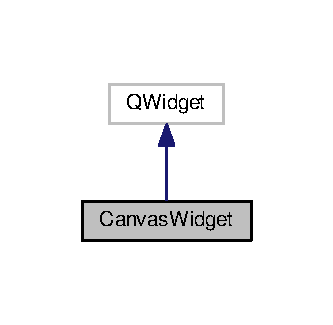
\includegraphics[width=160pt]{classCanvasWidget__inherit__graph}
\end{center}
\end{figure}


Collaboration diagram for Canvas\-Widget\-:\nopagebreak
\begin{figure}[H]
\begin{center}
\leavevmode
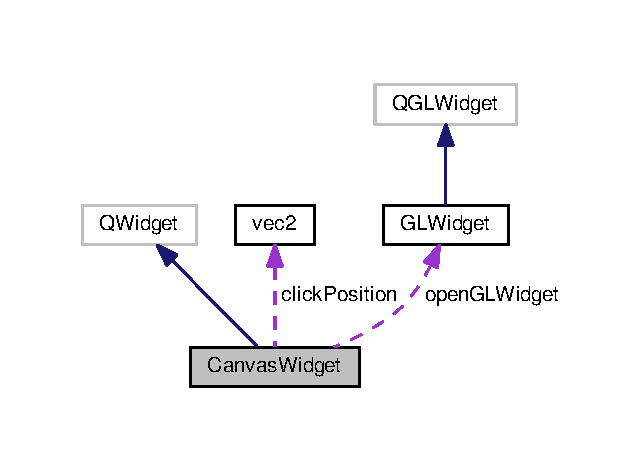
\includegraphics[width=309pt]{classCanvasWidget__coll__graph}
\end{center}
\end{figure}
\subsection*{Public Slots}
\begin{DoxyCompactItemize}
\item 
void \hyperlink{classCanvasWidget_a10d481976a36a4e489f42d2b5dfa4662}{change\-Tool} (int tool)
\item 
\hypertarget{classCanvasWidget_a24a75e8958b478656824d1d985d2d64d}{void {\bfseries open\-Color\-Picker} ()}\label{classCanvasWidget_a24a75e8958b478656824d1d985d2d64d}

\item 
\hypertarget{classCanvasWidget_a3dbc33d4382ea5295af8008760f123f3}{void {\bfseries set\-Current\-Color} (const Q\-Color \&color)}\label{classCanvasWidget_a3dbc33d4382ea5295af8008760f123f3}

\item 
\hypertarget{classCanvasWidget_a6a39b7120018202a7fc095a7638e8c90}{void {\bfseries deselect\-All} ()}\label{classCanvasWidget_a6a39b7120018202a7fc095a7638e8c90}

\item 
\hypertarget{classCanvasWidget_a692ef366f79d844dabc58803a82ba2d4}{void {\bfseries select\-All} ()}\label{classCanvasWidget_a692ef366f79d844dabc58803a82ba2d4}

\item 
\hypertarget{classCanvasWidget_afd4a461b8779e2d692a08647e655bc1e}{void {\bfseries zoom\-In} ()}\label{classCanvasWidget_afd4a461b8779e2d692a08647e655bc1e}

\item 
\hypertarget{classCanvasWidget_a0a19a82e3f4fbe354b779ff014e55ff2}{void {\bfseries zoom\-Out} ()}\label{classCanvasWidget_a0a19a82e3f4fbe354b779ff014e55ff2}

\item 
\hypertarget{classCanvasWidget_a05e567b5107bad5938e32a650c7696a6}{void {\bfseries update\-Size} ()}\label{classCanvasWidget_a05e567b5107bad5938e32a650c7696a6}

\item 
\hypertarget{classCanvasWidget_a9617418393fa64b4d662c0523acd98a2}{void {\bfseries undo} ()}\label{classCanvasWidget_a9617418393fa64b4d662c0523acd98a2}

\item 
\hypertarget{classCanvasWidget_ae6032a56c6be372d9b48fea14dcb1954}{void {\bfseries redo} ()}\label{classCanvasWidget_ae6032a56c6be372d9b48fea14dcb1954}

\item 
\hypertarget{classCanvasWidget_a0ccbb1b2140e5bbadc21ffe0684bd848}{void {\bfseries open} (std\-::string file\-Name)}\label{classCanvasWidget_a0ccbb1b2140e5bbadc21ffe0684bd848}

\item 
\hypertarget{classCanvasWidget_ac7465ba42b77a5a9a36af19073e0279a}{void {\bfseries save\-As} (std\-::string file\-Name)}\label{classCanvasWidget_ac7465ba42b77a5a9a36af19073e0279a}

\end{DoxyCompactItemize}
\subsection*{Signals}
\begin{DoxyCompactItemize}
\item 
\hypertarget{classCanvasWidget_a40301a55d3c5c4af8fdbb9a70942055c}{void {\bfseries color\-Changed} (const Q\-String \&style\-Sheet)}\label{classCanvasWidget_a40301a55d3c5c4af8fdbb9a70942055c}

\item 
\hypertarget{classCanvasWidget_ac2e5cfa7aac9658bf358af1e9b15d99e}{void {\bfseries state\-Changed} ()}\label{classCanvasWidget_ac2e5cfa7aac9658bf358af1e9b15d99e}

\end{DoxyCompactItemize}
\subsection*{Public Member Functions}
\begin{DoxyCompactItemize}
\item 
\hypertarget{classCanvasWidget_a3056d84c95e47f825ab4be09f48c0662}{{\bfseries Canvas\-Widget} (Q\-Widget $\ast$parent=0)}\label{classCanvasWidget_a3056d84c95e47f825ab4be09f48c0662}

\item 
\hypertarget{classCanvasWidget_a990d94414822524b183a4d90330ab13b}{int {\bfseries get\-Current\-Tool} ()}\label{classCanvasWidget_a990d94414822524b183a4d90330ab13b}

\end{DoxyCompactItemize}
\subsection*{Protected Member Functions}
\begin{DoxyCompactItemize}
\item 
\hypertarget{classCanvasWidget_a06806e2eda021c884160067a4148dc32}{void {\bfseries resize\-Event} (Q\-Resize\-Event $\ast$event)}\label{classCanvasWidget_a06806e2eda021c884160067a4148dc32}

\item 
\hypertarget{classCanvasWidget_a635c9e389dcdcc25cf218150b6c8a5cc}{void {\bfseries paint\-Event} (Q\-Paint\-Event $\ast$)}\label{classCanvasWidget_a635c9e389dcdcc25cf218150b6c8a5cc}

\item 
\hypertarget{classCanvasWidget_ab3ec45e42dd3da00012f3fb3e01666d4}{void {\bfseries mouse\-Press\-Event} (Q\-Mouse\-Event $\ast$event)}\label{classCanvasWidget_ab3ec45e42dd3da00012f3fb3e01666d4}

\item 
\hypertarget{classCanvasWidget_aa1ddd11ddeb07b7d4f105bf2959ce9bf}{void {\bfseries mouse\-Release\-Event} (Q\-Mouse\-Event $\ast$event)}\label{classCanvasWidget_aa1ddd11ddeb07b7d4f105bf2959ce9bf}

\item 
\hypertarget{classCanvasWidget_a1f0eced3fa450e2a04239b4fe8e3810a}{void {\bfseries mouse\-Move\-Event} (Q\-Mouse\-Event $\ast$event)}\label{classCanvasWidget_a1f0eced3fa450e2a04239b4fe8e3810a}

\end{DoxyCompactItemize}
\subsection*{Private Member Functions}
\begin{DoxyCompactItemize}
\item 
\hypertarget{classCanvasWidget_a4d553688bfcfc791d640d36587f27c26}{bool {\bfseries event\-Filter} (Q\-Object $\ast$object, Q\-Event $\ast$event)}\label{classCanvasWidget_a4d553688bfcfc791d640d36587f27c26}

\end{DoxyCompactItemize}
\subsection*{Private Attributes}
\begin{DoxyCompactItemize}
\item 
\hypertarget{classCanvasWidget_ad2353cc7b274a6db64eb6229fde95164}{\hyperlink{classGLWidget}{G\-L\-Widget} $\ast$ {\bfseries open\-G\-L\-Widget}}\label{classCanvasWidget_ad2353cc7b274a6db64eb6229fde95164}

\item 
\hypertarget{classCanvasWidget_aa66106798f5355101d44e8c095956cbe}{float {\bfseries zoom}}\label{classCanvasWidget_aa66106798f5355101d44e8c095956cbe}

\item 
\hypertarget{classCanvasWidget_ae3ca83bf96327e9a7ac8f9b85a07a292}{Q\-Color\-Dialog {\bfseries color\-Picker}}\label{classCanvasWidget_ae3ca83bf96327e9a7ac8f9b85a07a292}

\item 
\hypertarget{classCanvasWidget_a4ef50e03625f3d3343ebaabcb6ae93e7}{\hyperlink{classGLWidget_a9fba3eba78950865febd4547be0641d0}{G\-L\-Widget\-::\-Draw\-Tool} {\bfseries current\-Tool}}\label{classCanvasWidget_a4ef50e03625f3d3343ebaabcb6ae93e7}

\item 
\hypertarget{classCanvasWidget_a04b6116842600139d6c67d52dd118fcb}{Q\-Color {\bfseries current\-Color}}\label{classCanvasWidget_a04b6116842600139d6c67d52dd118fcb}

\item 
\hypertarget{classCanvasWidget_aefda1f3eaadbd5788e98f58e572d70b5}{\hyperlink{classvec2}{vec2} {\bfseries click\-Position}}\label{classCanvasWidget_aefda1f3eaadbd5788e98f58e572d70b5}

\item 
\hypertarget{classCanvasWidget_a40257c6897003c90e13cac2e97d644c9}{Q\-Widget $\ast$ {\bfseries main\-Window}}\label{classCanvasWidget_a40257c6897003c90e13cac2e97d644c9}

\item 
\hypertarget{classCanvasWidget_a6370f81145582e8583aca8c65c77be1c}{std\-::string {\bfseries m\-\_\-file\-Name}}\label{classCanvasWidget_a6370f81145582e8583aca8c65c77be1c}

\end{DoxyCompactItemize}


\subsection{Member Function Documentation}
\hypertarget{classCanvasWidget_a10d481976a36a4e489f42d2b5dfa4662}{\index{Canvas\-Widget@{Canvas\-Widget}!change\-Tool@{change\-Tool}}
\index{change\-Tool@{change\-Tool}!CanvasWidget@{Canvas\-Widget}}
\subsubsection[{change\-Tool}]{\setlength{\rightskip}{0pt plus 5cm}void Canvas\-Widget\-::change\-Tool (
\begin{DoxyParamCaption}
\item[{int}]{tool}
\end{DoxyParamCaption}
)\hspace{0.3cm}{\ttfamily [slot]}}}\label{classCanvasWidget_a10d481976a36a4e489f42d2b5dfa4662}
Changes the current tool being used to update the widget. This function calls G\-L\-Widget\-::change\-Tool(int) on the underlying \hyperlink{classGLWidget}{G\-L\-Widget}.


\begin{DoxyParams}{Parameters}
{\em tool} & A \hyperlink{classGLWidget_a9fba3eba78950865febd4547be0641d0}{G\-L\-Widget\-::\-Draw\-Tool} enum that represents the tool the widget should use.\\
\hline
\end{DoxyParams}
\begin{DoxySeeAlso}{See Also}
Canvas\-Widget\-::mouse\-Press\-Event(\-Q\-Event$\ast$) 

Canvas\-Widget\-::mouse\-Move\-Event(\-Q\-Event$\ast$) 

G\-L\-Widget\-::change\-Tool(int) 
\end{DoxySeeAlso}


The documentation for this class was generated from the following files\-:\begin{DoxyCompactItemize}
\item 
src/canvaswidget.\-hpp\item 
src/canvaswidget.\-cpp\end{DoxyCompactItemize}

\input{structBixelGrid_1_1HistoryState}
\hypertarget{classSwatch}{\section{Swatch Class Reference}
\label{classSwatch}\index{Swatch@{Swatch}}
}


Inheritance diagram for Swatch\-:\nopagebreak
\begin{figure}[H]
\begin{center}
\leavevmode
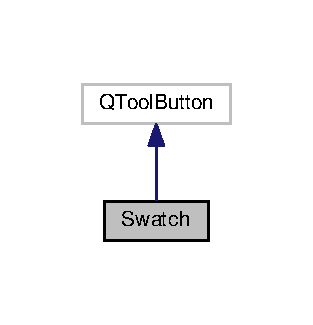
\includegraphics[width=150pt]{classSwatch__inherit__graph}
\end{center}
\end{figure}


Collaboration diagram for Swatch\-:\nopagebreak
\begin{figure}[H]
\begin{center}
\leavevmode
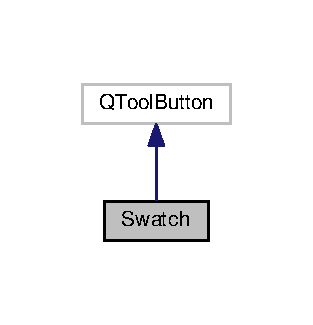
\includegraphics[width=150pt]{classSwatch__coll__graph}
\end{center}
\end{figure}
\subsection*{Signals}
\begin{DoxyCompactItemize}
\item 
\hypertarget{classSwatch_a4cc4620ddd05270f7c9a11addefcad57}{void {\bfseries swatch\-Picked} (const Q\-Color \&color)}\label{classSwatch_a4cc4620ddd05270f7c9a11addefcad57}

\end{DoxyCompactItemize}
\subsection*{Public Member Functions}
\begin{DoxyCompactItemize}
\item 
\hypertarget{classSwatch_ad411aab2ef21c65041939bfe3fe77b0e}{{\bfseries Swatch} (Q\-Widget $\ast$parent=0)}\label{classSwatch_ad411aab2ef21c65041939bfe3fe77b0e}

\item 
\hypertarget{classSwatch_a306fa88806e4b2d1fbf4e70f5878ae52}{void {\bfseries set\-Color} (Q\-Rgb color)}\label{classSwatch_a306fa88806e4b2d1fbf4e70f5878ae52}

\item 
\hypertarget{classSwatch_a53bfaa32646c4ee3555419f1edb5820d}{void {\bfseries set\-Color} (Q\-Color color)}\label{classSwatch_a53bfaa32646c4ee3555419f1edb5820d}

\item 
\hypertarget{classSwatch_aea70e9f1fd2b26b3e686b615b734d27a}{void {\bfseries set\-Color} (int r, int g, int b, int a=255)}\label{classSwatch_aea70e9f1fd2b26b3e686b615b734d27a}

\item 
\hypertarget{classSwatch_a6104b4c53efb97a496dd3554bf542ebb}{Q\-Color {\bfseries color} ()}\label{classSwatch_a6104b4c53efb97a496dd3554bf542ebb}

\end{DoxyCompactItemize}
\subsection*{Protected Member Functions}
\begin{DoxyCompactItemize}
\item 
\hypertarget{classSwatch_ab9aacb2c821dce15d22f54d34b68d023}{void {\bfseries mouse\-Release\-Event} (Q\-Mouse\-Event $\ast$)}\label{classSwatch_ab9aacb2c821dce15d22f54d34b68d023}

\end{DoxyCompactItemize}
\subsection*{Private Attributes}
\begin{DoxyCompactItemize}
\item 
\hypertarget{classSwatch_ac7c3eb52b20545b969f7aea97c985d5d}{Q\-Color {\bfseries m\-\_\-color}}\label{classSwatch_ac7c3eb52b20545b969f7aea97c985d5d}

\end{DoxyCompactItemize}


The documentation for this class was generated from the following files\-:\begin{DoxyCompactItemize}
\item 
src/swatch.\-hpp\item 
src/swatch.\-cpp\end{DoxyCompactItemize}

\hypertarget{classvec2}{\section{vec2 Class Reference}
\label{classvec2}\index{vec2@{vec2}}
}
\subsection*{Public Member Functions}
\begin{DoxyCompactItemize}
\item 
\hypertarget{classvec2_add5c0b4c7cf081d3292788a452cb489a}{{\bfseries vec2} (double x=0, double y=0)}\label{classvec2_add5c0b4c7cf081d3292788a452cb489a}

\item 
\hypertarget{classvec2_aedc685aecce22ebb9832a0dfa9ba4e76}{void {\bfseries set} (double x, double y)}\label{classvec2_aedc685aecce22ebb9832a0dfa9ba4e76}

\item 
\hypertarget{classvec2_a6e4d7583e07fd84b3314896e2f49f9c0}{\hyperlink{classvec2}{vec2} {\bfseries operator+} (const \hyperlink{classvec2}{vec2} \&b) const }\label{classvec2_a6e4d7583e07fd84b3314896e2f49f9c0}

\item 
\hypertarget{classvec2_afb69e05f24446157113eebf78b8fa64b}{\hyperlink{classvec2}{vec2} {\bfseries operator-\/} (const \hyperlink{classvec2}{vec2} \&b) const }\label{classvec2_afb69e05f24446157113eebf78b8fa64b}

\item 
\hypertarget{classvec2_aa9aacd2fc0ad8e81efe83e9f02b21749}{bool {\bfseries operator==} (const \hyperlink{classvec2}{vec2} \&b) const }\label{classvec2_aa9aacd2fc0ad8e81efe83e9f02b21749}

\end{DoxyCompactItemize}
\subsection*{Public Attributes}
\begin{DoxyCompactItemize}
\item 
\hypertarget{classvec2_ac38b8dcc3bc5eb2b4fb6971638af64d1}{double {\bfseries x}}\label{classvec2_ac38b8dcc3bc5eb2b4fb6971638af64d1}

\item 
\hypertarget{classvec2_a77fcc56ac7af5cee53b8ca789dacac1f}{double {\bfseries y}}\label{classvec2_a77fcc56ac7af5cee53b8ca789dacac1f}

\end{DoxyCompactItemize}


The documentation for this class was generated from the following files\-:\begin{DoxyCompactItemize}
\item 
src/vec2.\-hpp\item 
src/vec2.\-cpp\end{DoxyCompactItemize}

%--- End generated contents ---

% Index
\newpage
\phantomsection
\addcontentsline{toc}{chapter}{Index}
\printindex

\end{document}
